% thesis.tex -- 論文の書き方参考例
%
% (注意)氏名、学籍番号等を変更すること。
%
% (LaTeXの実行法) platex thesis.tex
%
%	このファイル内にある '% 'はコメント。
%
\documentclass[a4j,11pt]{jreport}
\usepackage{ascmac}
\usepackage{amsmath}
\usepackage{float}
\usepackage{url}
\usepackage[dvipdfmx]{graphicx}
\usepackage{thesis-master}
\usepackage{mylatex}
\pagestyle{plain}

% 所属研究科、専攻
\courseofmastercs
% 研究テーマ
\title{}
% 氏名
\author{吉田健太}
% 学籍番号
\id{G2116032}
% 指導教員
\teacher{木下 俊之}
% 提出日
\date{2018}{1}{23}
% 提出年度
\schoolyear{2017}

% 研究室名(カバー用)
\clab{木下}
% 学籍番号(カバー用)
\cid{G2116032}

%% 英語要旨
\etitle{Cost reduction for initial learning using analogy traffic of machine learning}
\eauthor{Kenta Yoshida}
\eteacher{Kinoshita Toshiyuki}

\begin{document}
\makecover		% カバー
\maketitle		% 表紙

% 修士論文日本語概要
\jabst{
% abstract.tex -- 論文概要
現行IntrusionDet tionSystem (IDS)にはアノマリ型とシグネチャ型が存在している。
パターンファイルをセッティングするシグネチャ型は既存攻撃には強いが未知攻撃や亜種攻撃に対しては検知できない課題がある。
そこで未知攻撃や亜種攻撃に対して検出するためのアノマリ型がIDSが注目を集めている。
しかし実環境において稼働に耐える学習データを生成するデータ量を確保するには多大な時間的コストがかかることが問題となっている。
本研究では類似するネットワークからキャプチャーしたネットワークデータを用いて学習にかかる時間的コストの削減を提案する。
より実環境に近い状態を想定して脆弱性スキャナ及び実ネットワークのトラフィックを用いて評価を行う。
なお、検知対象としてHTTPにおける攻撃に注目しており、プロトコルはHTTP限定する。
	% abstract.texを読み込む
}
\makejabstract

% 修士論文英語概要
\eabst{
% abstract.tex -- 論文概要
Write an abstract of your Paper.

}
\makeeabstract

% 目次
\pagenumbering{roman}
\setcounter{page}{1}
\thispagestyle{plain}
\tableofcontents	% 目次
\listoffigures		% 図目次
\listoftables		% 表目次
%\listofprograms		% プログラム目次

% 論文本文
%   論文本文は章や節単位で,いくつかのファイルに分割したほうが編集しやすい.
% \input{hogehoge}	% hogehoge.texを読み込む.
% 章構成は適宜変更すること.
\pagenumbering{arabic}
\chapter{はじめに}
\section{はじめに}
本テンプレートは東京工科大学大学院\cite{teu}のバイオ・情報メディア研究科
コンピュータサイエンス専攻の修士論文用に作成されました.以下にテンプレー
トの使い方を簡単に説明していきます.また,{\TeX}全般に関する使い方は,奥
村先生の美文書作成入門\cite{okumura}を参考にしてください.

\section{論文情報の登録}
thesis.tex を開くと,ファイル上部に``\verb|\title{論文タイトル}|''や
``\verb|\author{工~~科~~~太~~郎}|''など論文の情報を入力する箇所があります.
まずは,これらの情報を自身のものに適宜変更してください.本テンプレートで
は入力された情報から``受領書''や``ファイルのカバー'',``内表紙'',``概
要'',``英語要旨''を作成しますので,間違えないように気をつけて入力してく
ださい.

\section{本テンプレートで用意したコマンド}
本テンプレートでは図や表を参照するためのコマンドを用意しました.

\subsection{図の例}
図の参照には\verb|\figref{}|を用います.このコマンドは,図を参照する際に
``図''という文字を自動的に付与します.また,1回目の参照では\textbf{太字}
で表示し,2回目以降は通常表示します.

例)本学園の校章を\figref{fig:teu}に示す.
\begin{figure}[tb]
 \centering
 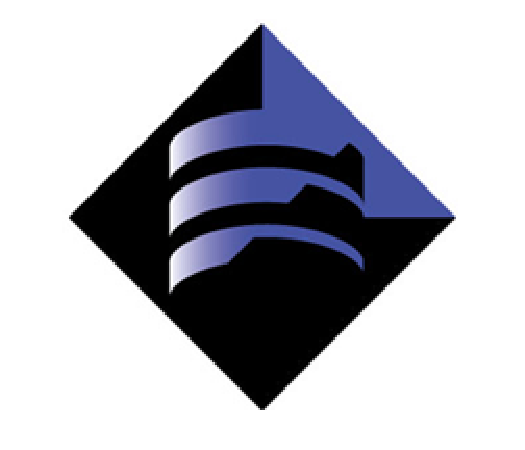
\includegraphics[clip, width=0.5\linewidth]{teulogo_new.eps}
  \caption{本学園の校章}
 \label{fig:teu}
\end{figure}

\subsection{表の例}
表の参照には\verb|\tabref{}|を用います.このコマンドは,表を参照する際に
``表''という文字を自動的に付与します.また,1回目の参照では\textbf{太字}
で表示し,2回目以降は通常表示します.

例)東京工科大学の学部別の学生数をまとめた表を\tabref{tab:teu}に示す.
\begin{table}[tb]
 \begin{center}
  \caption{学部別の人数(2009年5月1日現在)} \label{tab:teu}
  \begin{tabular}{l|c|c|c}\hline\hline
   学部 & 男子(名) & 女子(名) & 合計(名)\\\hline
   メディア学部 & 1618 & 553 & 2151\\
   応用生物学部 & 1081 & 417 & 1498\\
   コンピュータサイエンス学部 & 2046 & 146 & 2192\\ \hline
  \end{tabular}
 \end{center}
\end{table}

\subsection{式の例}
式の参照には\verb|\eqref{}|を用います.このコマンドは,式を参照する際に
``式''という文字を自動的に付与します.また,1回目の参照では\textbf{太字}
で表示し,2回目以降は通常表示します.

例)オイラーの公式を\eqref{eq:euler}に示す.
\begin{equation}
 e^{i\theta} = \cos\theta + i \sin\theta\label{eq:euler}
\end{equation}

\subsection{プログラムの例}
プログラムの参照には\verb|\pgref{}|を用います.このコマンドは,プログラム
を参照する際に``プログラム''という文字を自動的に付与します.また,1回目の
参照では\textbf{太字} で表示し,2回目以降は通常表示します.

例)プログラムの表示の方法には2種類あります.1つは,外部に保存したファイル
を読み込んで表示する方法です.もう1つは,直接プログラムを記述する方法で
す.

``Hello World''を表示するCのプログラムを\pgref{pg:helloc}に示す.
\lstinputlisting[caption=Hello World, label=pg:helloc,
language=c]{hello.c}

``Hello Java''を表示するJavaのプログラムを\pgref{pg:hellojava}に示す.
\begin{lstlisting}[caption=Hello Java, label=pg:hellojava,language=java]
 public class HelloJava {
     public static void main(String[] args) {
         System.out.println("Hello Java");
     }
 }
\end{lstlisting}
		% 第1章 はじめに
\chapter{関連技術}

\section{重複除外}

\subsection{シングルスタック}

\subsection{固定長ブロック法}

\subsection{可変長ブロック法}


\section{Hash}

\subsection{SHA-1}

\subsection{MD5}

\section{OpenCV}

\section{image File}

\subsection{フォーマット}
		% 第2章 関連技術
\chapter{提案}
\section{システムの全体説明}
\subsection{正規通信の収集・加工方法}
\subsection{学習データの統合}
\section{クライアント側での運用}
	% 第3章 提案
\chapter{例: 実装}
章立ては指導教員の方針に従ってください.
	% 第4章 実装
\chapter{例: 評価}
章立ては指導教員の方針に従ってください.
	% 第5章 評価
\chapter{評価}
\section{結果概要}
	% 第6章 おわりに
% acknowlegments.tex -- 謝辞
\theacknowledgments
本論文の作成にあたり、終始適切な助言を賜り、また丁寧に指導して下さった木下 俊之先生にこの場を借りて感謝の意を表します。
		% 謝辞
\bibliographystyle{junsrt}
\bibliography{mybib}
% appendix.tex -- 付録
\appendix
\chapter{ソースコード}
\section{CONTENT}
リストファイルを\pgref{pg:CONTENT}に示す.

\lstinputlisting[caption=CONTENT,
label=pg:CONTENT]{00CONTENT}
	% 付録
\end{document}
